%%%%%%%%%%%%%%%%%%%%

% Homework: Autoignition &Knock in
% Spark Ignition Engines
% Pradip Xavier - Bruno Renou
% pradip.xavier@insa-rouen.fr
% Energy Engineering Department, 2023-2024
% Important notes:
% • Read carefully the questions. During writing, pay attention to clearly state all
% hypothesis and to be pedagogical enough.
% •You can write either in French or English (no page limitations).
% •Estimated working load estimated: 2h (in exam conditions).
% •Work to be submitted on moodle or at my office by 08/12/2023, 23h59.
% Industrial problem
% Internal combustion (IC) engines are widely used as individual transportation means all around the
% world. Environmental concerns (i.e. climate change) raise new challenges to develop highly efficient
% and clean engines to absorb the future demand for cars (forecasts announce 2 billion cars in 2040, being
% twice than current figures1). Fuel flexibility is a crucial criterion: it consists in having an engine that
% operates with different types of fuels. Unfortunately, engine knock is currently limiting the efficiency
% of such engines. Knock is caused by an autoignition of local ”hot spots” in the fresh gases (ahead
% of the flame front), leading to multiple ignition areas and high pressure gradient in the engine. This
% homework aims to develop a simple yet predictive model to estimate autoignition in IC engines.
% Development of a model to predict autoignition
% The development of the model will be made from local equations governing the combustion process in
% order to determine auto-ignition by-hand. Many assumptions (e.g. one-step chemistry) will be made.
% 1) Draw the PV cycle of a spark ignition engine fueled with gasoline. What are the thermodynamic
% conditions (P, T, V) during the combustion process?
% 2) Identify a a simple control volume to study the combustion process in IC engines. Write the
% first law of thermodynamics on the chosen system and by assuming that the problem is only
% time-dependent. Show that the differential equation can be written as
% du
% dt = 1
% m
% d
% dt(
% N∑
% k
% nkumk ) =  ̇Q
% m (1)
% u is the mixture internal energy per unit of mass, m is the total mass of the mixture made of N
% species, nk is the number of moles of species k, umk is the molar internal energy of species k and ̇Q is the power exchanged by the system with its environment.
% 1BP Energy Outlook 2018 Edition, www.bp.com
% 1
% 3) Expand Eq. 1 by introducing the molar reaction rate of species k,  ̇ωmk (i.e. rate of production/-
% consumption of a species), the molar heat capacity at constant volume of species k, Cmv,k and the
% concentration of species k, [Xk].
% 4) Modify the expression found in 3) by introducing the molar enthalpy of species k, hmk and the
% molar heat capacity of species k at constant pressure, Cmp,k. Show that the time derivative of
% temperature can be expressed as
% dT
% dt =  ̇Q/V + RT ∑N
% k  ̇ωmk −∑N
% k hmk  ̇ωmk∑N
% k [Xk](Cmp,k −R) (2)
% 5) Apply the perfect gas law to a mixture made of N species. Differentiate the pressure with time
% in the case of a constant volume combustion and by introducing the reaction rate  ̇ωmk and the
% concentration [Xk] of a species k. Then, show that the time derivative of pressure is
% dP
% dt = RT
% N∑
% k
%  ̇ωmk + R
% N∑
% k
% [Xk] dT
% dt (3)
% What is the condition required to neglect the first term of the right-hand side?
% 6) The set of equations derived in the previous questions will be applied into an IC engine operating
% with an ethane/air mixture. The combustion process will occur at lean/stoichiometric conditions
% and one single-step chemistry will be considered.
% a. Write the global combustion equation by using the theoretical amount of air, Va,0 and the
% excess air e. Calculate Va,0.
% b. By considering stoichiometric conditions, determine the molar mass of fuel, MF , oxidizer
% (i.e. the air), Mox, and combustion products MP r. Conclude.
% c. The one-step chemistry of ethane can be represented by the following form:
% d[F]
% dt = −1.1 ×1012e−15098/T [F]0.1[O2]1.65 = − ̇ωmF . (4)
% Provide simple expressions for d[O2]
% dt , d[ox]
% dt and d[P r]
% dt as a function of d[F ]
% dt .
% d. Assuming that:
% - molar heat capacity, Cmp , of fuel, oxidizer and products are identical and constant (i.e.
% not dependent on temperature),
% - formation enthalpy of oxidizer and products are approximated to 0,
% - the combustion chamber is adiabatic,
% plot qualitatively the enthalpy, hmk , of fuel, oxidizer and by-products in a H-T diagram.
% Show that Eqs. 2 and 3 can be simplified as
% dT
% dt ≈ −∆h0,m
% f,k  ̇ωmF
% (Cmp −R) P/RT dP
% dt = P
% T
% dT
% dt = P0
% T0
% dT
% dt (5)
% e. The initial temperature and pressure before combustion are 753 K and 25.12 atm, respec-
% tively. Calculate the molar concentrations [F]0, [O2]0 and [Pr]0.

%%%%%%%%%%%%%%%%%%%%


%!TEX encoding = UTF-8 Unicode
\documentclass[11pt, a4paper]{article} %twocolumn

\usepackage{amsfonts}
\usepackage{graphicx}
\usepackage{pifont}
\usepackage{wrapfig}
\usepackage{caption}
\usepackage{mathptmx}
\usepackage{amsmath,amssymb,bm}
\usepackage{tabularx}
\usepackage{graphicx}
\usepackage{multicol}
\usepackage{multirow}
\usepackage{float}
\usepackage{subcaption}
\usepackage{gensymb}
\usepackage{hyperref}

\usepackage[table]{xcolor}
\usepackage{caption,subcaption,enumitem}

\usepackage[french]{babel}		
\usepackage[utf8]{inputenc}
\usepackage[T1]{fontenc}
\usepackage{lmodern} 
\usepackage{amsmath}
\usepackage{esint}

\usepackage{geometry}
\geometry{hmargin=1.5cm, vmargin=2.8cm}

%%%%%%
\usepackage{parskip}
\setlength{\parskip}{10pt}


\usepackage{titlesec}
\titleformat{\section}{\Large\bfseries}{\thesection}{1em}{}
\titleformat{\subsection}{\large\bfseries}{\thesubsection}{1em}{}


\title{\textit{Combustion 2}\\
\vspace{1cm}
\hrule
\vspace{0.5cm}
\textbf{Homework: Autoignition \& Knock in Spark Ignition Engines}
\vspace{0.5cm}
\hrule}

\author{\textbf{Delamare Yanis}\\
~\\
Energétique \& Propulsion 4ème année - INSA Rouen Normandie}

\date{Année universitaire 2023-2024}

\usepackage{fancyhdr}
\pagestyle{fancy}
\fancyhf{}
\lhead{Homework: Autoignition \& Knock in Spark Ignition Engines}
\chead{}
\rhead{Delamare Yanis EP4}

\begin{document}

\maketitle
%\vspace{3cm}

\begin{figure}[H]
    \centering
    %\includegraphics[width=0.4\columnwidth]{pic.png}
    \caption{Pic}
\end{figure}

\maketitle\thispagestyle{empty}

%%%%%%
\vspace{0.1cm}

\begin{abstract}
    Blablabla
\end{abstract}


\newpage

\tableofcontents
%\listoffigures
\pagenumbering{arabic}


%%% INTRO %%%
\newpage
\fancyfoot[C]{\thepage}
\setcounter{page}{1}
\part{Introduction}


\section{Spark ignition engine cycle}

blabla

\section{Definition of the system and fist law of thermodynamics}

The control volume to study the combustion process in IC engines can be defined as the volume delimited by the piston, the cylinder head and the cylinder walls. 
We can make the assumption that the combustion chamber is adiabatic with a constant volume $dV = 0$ and that the combustion process is isochoric.

The first law of thermodynamics applied to the control volume gives:
\begin{equation}
    \Delta U = Q - W
\end{equation}

Here there is no work done by the system, so $W = 0$ since $dV = 0$. We can therefor write:

\begin{equation}
    \frac{dU}{dt} = \dot{Q} \iff \frac{du}{dt} = \frac{\dot{Q}}{m}
\end{equation}

We can decompose the internal energy by a sum of the internal energy of the different species in the control volume:

\begin{equation}
    u = \frac{1}{m} \sum_{k=1}^{N} n_k u_k^m
\end{equation}

Where $n_k$ is the number of moles of the species $k$ and $u_k^m$ is the molar internal energy of the species $k$.

We can then write:
\begin{equation}
    \boxed{
        \frac{du}{dt} = \frac{1}{m} \frac{d}{dt} \left( \sum_{k=1}^{N} n_k u_k^m \right) = \frac{\dot{Q}}{m}
    }
\end{equation}


\section{Introduction to the molar reaction rate and the molar heat capacity at constant volume}

\begin{equation}
    \dot{Q} = \frac{d}{dt} \left( \sum_{k=1}^{N} n_k u_k^m \right) = \sum_{k=1}^{N} \frac{dn_k}{dt} u_k^m + \sum_{k=1}^{N} n_k \frac{du_k^m}{dt}
\end{equation}

We know the following relation:


\begin{equation}
    \left[ X_k \right] = \frac{n_k}{V}
    \\
    \text{ and }
    \\
    \dot{\omega}_k^m = \frac{d \left[ X_k \right] }{dt} = \frac{d \left( n_k/V \right) }{dt} \iff \frac{dn_k}{dt} = \dot{\omega}_k^m V
\end{equation}

Where $\dot{\omega}_k^m$ is the molar production rate of the species $k$

\begin{equation}
    C^m_{v,k} = \frac{du_k^m}{dT} \iff \frac{du_k^m}{dt} = C^m_{v,k} \frac{dT}{dt}
\end{equation}

\begin{equation}
    \boxed{
        \frac{\dot{Q}}{V} = \sum_{k=1}^{N} \dot{\omega}_k^m u_k^m + \sum_{k=1}^{N} \left[ X_k \right] C^m_{v,k} \frac{dT}{dt}
    }
\end{equation}

\section{Introduction of the molar enthalpy and molar heat capacity at constant pressure}

Moreover, we know that:

\begin{equation}
    H = U + PV \iff h_k^m = u_k^m + RT
\end{equation}

\begin{equation}
    C_{p,k}^m - C_{v,k}^m = R
\end{equation}

So we can write:

\begin{equation}
    \frac{\dot{Q}}{V} = \sum_{k=1}^{N} \dot{\omega}_k^m h_k^m - RT \sum_{k=1}^{N} \dot{\omega}_k^m + \sum_{k=1}^{N} \left[ X_k \right] \left( C_{p,k}^m - R \right) \frac{dT}{dt}
\end{equation}

And we find the desired expression:


\begin{equation}
    \boxed{
        \frac{dT}{dt} = \frac{\dot{Q}/V + RT \sum_{k=1}^{N} \dot{\omega}_k^m - \sum_{k=1}^{N} \dot{\omega}_k^m h_k^m}{\sum_{k=1}^{N} \left[ X_k \right] \left( C_{p,k}^m - R \right)}
    }
\end{equation}


\section{Differentiation of the pressure with time with perfect gas assumption}

\begin{equation}
    P = \frac{nRT}{V}
    \iff
    \frac{dP}{dt} = \frac{nR}{V} \frac{dT}{dt} + \frac{RT}{V} \frac{d n }{dt}
\end{equation}

\begin{equation}
    \frac{dP}{dt} = \frac{nR}{V} \frac{dT}{dt} + \frac{RT}{V} \frac{d \sum_{k=1}^{N} n_k }{dt} = \frac{nR}{V} \frac{dT}{dt} + \frac{RT}{V} \sum_{k=1}^{N} \frac{d n_k }{dt} = \frac{nR}{V} \frac{dT}{dt} + \frac{RT}{V} \sum_{k=1}^{N} \dot{\omega}_k^m V
\end{equation}

We do finally find the next desired expression:

\begin{equation}
    \boxed{
        \frac{dP}{dt} = RT \sum_{k=1}^{N} \dot{\omega}_k^m + R \sum_{k=1}^{N} \left[ X_k \right] \frac{dT}{dt}
    }
\end{equation}

The condition required to neglect the term $RT \sum_{k=1}^{N} \dot{\omega}_k^m$ is:

\begin{equation}
    \sum_{k=1}^{N} \dot{\omega}_k^m \approx 0
\end{equation}


\section{Ethane/air mixture combustion}

\subsection{Global combustion equation}

\begin{equation}
    C_2H_6 + \frac{V_{a,0}}{4.76} \left( O_2 + 3.76 N_2 \right) \rightarrow A \cdot CO_2 + B \cdot H_2O + C \cdot N_2
\end{equation}

Equations of the different atoms:

\renewcommand{\arraystretch}{1.5}

\begin{center}
    \begin{tabular}{|c|>{\centering\arraybackslash}m{4cm}|>{\centering\arraybackslash}m{5cm}|}
        \hline
        Atom & Equation & Conclusion \\
        \hline
        H & $6 = 2B$ & $B = 3$ \\
        \hline
        N & $2 \cdot \frac{V_{a,0}}{4.76} \cdot 3.76 = 2 \cdot C$ & $C = \frac{V_{a,0}}{4.76} \cdot 3.76$ \\
        \hline
        O & $2 \cdot \frac{V_{a,0}}{4.76} = 2A + B$ & $A = \frac{V_{a,0}}{4.76} - \frac{3}{2}$ \\
        \hline
        C & $A = 2$ & $A = 2$ \\
        \hline
    \end{tabular}
\end{center}

So we have:

\begin{equation}
    2 = \frac{V_{a,0}}{4.76} - \frac{3}{2} \iff V_{a,0} = \left( 2 + \frac{3}{2} \right) \cdot 4.76
\end{equation}

\begin{equation}
    \boxed{
        V_{a,0} = 16.66
    }
\end{equation}

We can now write the global stoichiometric equation:

\begin{equation}
    \boxed{
        C_2H_6 + \frac{V_{a,0}}{4.76} \left( O_2 + 3.76 N_2 \right) \rightarrow 2 CO_2 + 3 H_2O + \frac{V_{a,0}}{4.76} \cdot 3.76 N_2
    }
\end{equation}

And the equation by introducing the excess air coefficient $e$:

\begin{equation}
    \boxed{
        C_2H_6 + \left( 1+e \right) \cdot \frac{V_{a,0}}{4.76} \left( O_2 + 3.76 N_2 \right) \rightarrow 2 CO_2 + 3 H_2O + \left( 1+e \right) \cdot \frac{V_{a,0}}{4.76} \cdot 3.76 N_2 + e \cdot \frac{V_{a,0}}{4.76} O_2
    }
\end{equation}


\subsection{Molar mass}

By using a small cantera python script, we found the molar mass of different species:

\begin{center}
    \begin{tabular}{|c|c|}
        \hline
        Species & Molar mass (g/mol) \\
        \hline
        Fuel $C_2H_6$ & 30.0700 \\
        \hline
        Air ($O_2$, $N_2$) & 28.8510 \\
        \hline
        Products ($CO_2$, $H_2O$, $N_2$, $O_2$) & 28.1237 \\
        \hline
    \end{tabular}
\end{center}

We can conclude that we can make the assumption that all the species have the same molar mass $M$ at the standard temperature and pressure.

\begin{figure}[H]
    \centering
    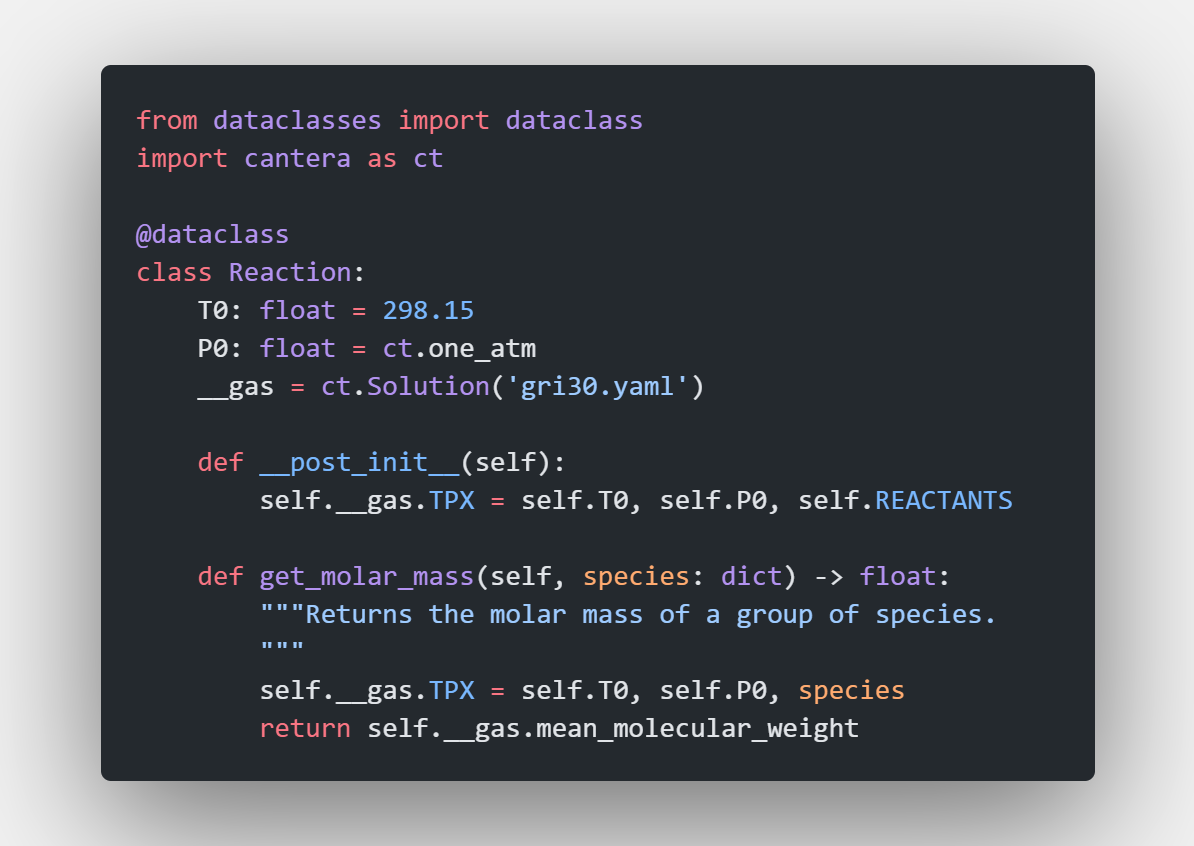
\includegraphics[width=0.6\linewidth]{images/mean_molecular_weight.png}
    \caption{Python script to compute the molar mass of different species}
    \label{fig:ethane_air_molar_mass}
\end{figure}

\subsection{One-step chemistry}

The one-step chemistry of ethane is the following:

\begin{equation}
    \frac{ d \left[ F \right] }{ dt } = - 1.1 \cdot 10^{12} \cdot e^{-15098/T} \cdot \left[ F \right]^{0.1} \cdot \left[ O_2 \right]^{1.65} = - \dot{\omega}_F^m
\end{equation}

We can therefore provide simple expression for one-step chemistry of air and products:

\begin{equation}
    \frac{ d \left[ O_2 \right] }{ dt } = \left( e \cdot \frac{V_{a,0}}{4.76} \right) \cdot \dot{\omega}_F^m
\end{equation}

\begin{equation}
    \frac{ d \left[ Air \right] }{ dt } = - \left( \left( 1 + e \right) \cdot \frac{V_{a,0}}{4.76} \cdot \left( 1 + 3.76 \right) \right) \cdot \dot{\omega}_F^m
\end{equation}

\begin{equation}
    \frac{ d \left[ Products \right] }{ dt } = \left( 2 + 3 + (1+e) \cdot 3.76 \frac{V_{a,0}}{4.76} + e \cdot \frac{V_{a,0}}{4.76} \right) \cdot \dot{\omega}_F^m
\end{equation}

\subsection{Simplification of the derivatives}


We can make the following simplifications:

\begin{itemize}

    \item $\dot{Q} = 0$ because we consider that the system is adiabatic.

    \item $\sum_{k=1}^{N_s} \dot{\omega}_k^m = 0$ as we proved earlier.

    \item $h_k^m = \int_{T_0}^{T} C^m_{p,k} dT + \Delta h_{f,k}^{0,m}$

    \item $\sum_{k=1}^{N} \left[ X_k \right] = 1$ because ...

\end{itemize}

Then we can write:

\begin{equation}
    \frac{ dT }{ dt } = - \frac{ \sum_{k=1}^{N} \int_{T_0}^{T} C^m_{p,k} dT + \Delta h_{f,k}^{0,m} \dot {\omega}_k^m } { \sum_{k=1}^{N} \left( C^m_{p,k} - R \right) }
\end{equation}

We have too:

\begin{itemize}
    \item Molar heat capacity of fuel, oxidizer and products are identical and constant.
    \item Formation enthalpy of oxidizer and products are approximated to 0.
\end{itemize}

Therefore:

\begin{equation}
    \frac{ dT }{ dt } = - \frac{ C^m_{p,k} \sum_{k=1}^{N} \int_{T_0}^{T} dT + \Delta h_{F,k}^{0,m} \dot {\omega}_F^m } { \left( C^m_{p} - R \right) }
\end{equation}

\subsection{Determine initial conditions}

Initial conditions are set up at a temperature of $T_0 = 753 K$ and a pressure of $P_0 = 25.12 atm$.

We initially have:

\begin{equation}
    \left[ X_k \right] = \frac{n_k}{V}
\end{equation}

By using the ideal gas law, we can write:

\begin{equation}
    P_k \cdot V = n_k RT \iff n_k  = \frac{P_k \cdot V}{R \cdot T}
\end{equation}

Therefore:

\begin{equation}
    \left[ X_k \right] = \frac{P_k}{R \cdot T} = X_k \cdot \frac{P}{R \cdot T} = \frac{n_k}{n_{tot}} \cdot \frac{P}{R \cdot T}
\end{equation}

To conclude we can determine the initial conditions of the different species:

\begin{equation}
    \boxed{
        \left[ X_k \right]_0 = \frac{n_{k,0}}{n_{tot}} \cdot \frac{P_0}{R \cdot T_0}
    }
\end{equation}

\begin{equation}
    \left[ F \right]_0 = \frac{n_{F,0}}{n_{tot}} \cdot \frac{P_0}{R \cdot T_0} = \frac{1}{1 + \left( (1+e) \cdot \frac{V_{a,0}}{4.76} \cdot (1+3.76) \right)} \cdot \frac{P_0}{R \cdot T_0} \approx 0.0566 \cdot \frac{P_0}{R \cdot T_0} \approx 23.049 \text{ } mol/m^3
\end{equation}

\begin{equation}
    \left[ O_2 \right]_0 = \frac{n_{O_2,0}}{n_{tot}} \cdot \frac{P_0}{R \cdot T_0} = \frac{(1+e) \cdot \frac{V_{a,0}}{4.76}}{1 + \left( (1+e) \cdot \frac{V_{a,0}}{4.76} \cdot (1+3.76) \right)} \cdot \frac{P_0}{R \cdot T_0} \approx 0.1982 \cdot \frac{P_0}{R \cdot T_0} \approx 80.673 \text{ } mol/m^3
\end{equation}

\begin{equation}
    \left[ Products \right]_0 = \frac{n_{Products,0}}{n_{tot}} \cdot \frac{P_0}{R \cdot T_0} = 0 \text{ } mol/m^3
\end{equation}



\newpage
\part{Python application}


\newpage
\part*{Annexes}
\appendix
\section{Code}



\end{document}
